\documentclass[11pt,letterpaper]{article}
\usepackage{../acl2015}
\usepackage{times}
\usepackage{latexsym}
% \setlength\titlebox{7.5cm}    % Expanding the titlebox

%%% Custom additions %%%
\usepackage{url}
\usepackage[leqno, fleqn]{amsmath}
\usepackage{amssymb}
\usepackage{qtree}
\usepackage{graphicx} 
\usepackage{booktabs}
\usepackage{multirow}
\usepackage{colortbl}
\usepackage{caption}
\usepackage{subcaption}
\usepackage{color}
\usepackage{xcolor}
\usepackage{tikz}
\usepackage{tikz-qtree}
\usepackage{pgfplots}
\usepackage{ifthen}
\usepackage{framed}
\usepackage{algorithm}
\usepackage[noend]{algpseudocode}

\newcommand\todo[1]{\textcolor{blue}{\textbf{TODO:} #1}}
\newcommand\result[1]{\textcolor{red}{\textbf{RESULT NEEDED:} #1}}
\newcommand\question[1]{\textcolor{orange}{\textbf{OPEN QUESTION:} #1}}

\newcount\colveccount
\newcommand*\colvec[1]{
        \global\colveccount#1
        \begin{bmatrix}
        \colvecnext
}
\def\colvecnext#1{
        #1
        \global\advance\colveccount-1
        \ifnum\colveccount>0
                \\
                \expandafter\colvecnext
        \else
                \end{bmatrix}
        \fi
}

\newcommand{\nateq}{\equiv}
\newcommand{\natind}{\mathbin{\#}}
\newcommand{\natneg}{\mathbin{^{\wedge}}}
\newcommand{\natfor}{\sqsubset}
\newcommand{\natrev}{\sqsupset}
\newcommand{\natalt}{\mathbin{|}}
\newcommand{\natcov}{\mathbin{\smallsmile}}

\newcommand{\plneg}{\mathop{\textit{not}}}
\newcommand{\pland}{\mathbin{\textit{and}}}
\newcommand{\plor}{\mathbin{\textit{or}}}

\newcommand{\shift}{\textsc{shift}}
\newcommand{\reduce}{\textsc{reduce}}

% Strikeout
\newlength{\howlong}\newcommand{\strikeout}[1]{\settowidth{\howlong}{#1}#1\unitlength0.5ex%
\begin{picture}(0,0)\put(0,1){\line(-1,0){\howlong\divide\unitlength}}\end{picture}}

\newcommand{\True}{\texttt{T}}
\newcommand{\False}{\texttt{F}}
\usepackage{stmaryrd}
\newcommand{\sem}[1]{\ensuremath{\llbracket#1\rrbracket}}

\newcommand{\mynote}[1]{{\color{blue}#1}}
\newcommand{\tbchecked}[1]{{\color{red}#1}}

\usepackage{gb4e}
\noautomath
 
\def\ii#1{\textit{#1}}
\newcommand{\word}[1]{\emph{#1}}
\newcommand{\fulllabel}[2]{\b{#1}\newline\textsc{#2}}


%%%%%%%%%%%%%%%%%%%%%%%%%%%%%%%%%%%%%%%%%%%%%%%%%%%%%%%%%%%%%%%%%%%%%%
%%%%% Code to simulate natbib's citealt, which prints citations with
%%%%% no parentheses:

\makeatletter
\def\citealt{\def\citename##1{{\frenchspacing##1} }\@internalcitec}
\def\@citexc[#1]#2{\if@filesw\immediate\write\@auxout{\string\citation{#2}}\fi
  \def\@citea{}\@citealt{\@for\@citeb:=#2\do
    {\@citea\def\@citea{;\penalty\@m\ }\@ifundefined
       {b@\@citeb}{{\bf ?}\@warning
       {Citation `\@citeb' on page \thepage \space undefined}}%
{\csname b@\@citeb\endcsname}}}{#1}}
\def\@internalcitec{\@ifnextchar [{\@tempswatrue\@citexc}{\@tempswafalse\@citexc[]}}
\def\@citealt#1#2{{#1\if@tempswa, #2\fi}}
\makeatother

%%%%%%%%%%%%%%%%%%%%%%%%%%%%%%%%%%%%%%%%%%%%%%%%%%%%%%%%%%%%%%%%%%%%%

\title{A fast unified model for parsing and sentence understanding} 

%     \author{}
    \author{
    Samuel R.\ Bowman$^{1,2,5,}$\thanks{~\,The first two authors contributed equally.} \\
    \texttt{\small sbowman@stanford.edu} \\
    \And
    Jon Gauthier$^{2,3,5,*}$ \\
    \texttt{\small jgauthie@stanford.edu} \\
    \And
    Abhinav Rastogi$^{4,5}$ \\
    \texttt{\small arastogi@stanford.edu} \\
    \AND
    Raghav Gupta$^{6}$ \\
    \texttt{\small rgupta93@stanford.edu} \\
    \And
    Christopher D.\ Manning$^{1,2,5,6}$\\
    \texttt{\small manning@stanford.edu}\\
    \And
    Christopher Potts$^{1}$\\
    \texttt{\small cgpotts@stanford.edu}
    \AND\\[-3ex]
    {$^{1}$Stanford Linguistics\quad
    $^{2}$Stanford NLP Group\quad
    $^{3}$Stanford Symbolic Systems}\\
    {$^{4}$Stanford Electrical Engineering\quad
    $^{5}$Stanford AI Lab\quad
    $^{6}$Stanford Computer Science}
    }

\date{}

\makeatletter
\newcommand{\@BIBLABEL}{\@emptybiblabel}
\newcommand{\@emptybiblabel}[1]{}
\definecolor{black}{rgb}{0,0,0}
\makeatother
\usepackage[breaklinks, colorlinks, linkcolor=black, urlcolor=black, citecolor=black, draft]{hyperref}

\def\t#1{#1}
\def\b#1{\t{\textbf{#1}}}
\def\colspaceS{2.25mm}
\def\colspaceM{4.0mm}
\def\colspaceL{4.25mm}

\begin{document}
\maketitle
\begin{abstract}

Tree-structured neural networks exploit valuable syntactic parse information as they interpret the meanings of sentences. However, they suffer two key technical problems: they can only operate on parsed sentences and do not directly support batched computation, making them slow and unwieldy for large-scale NLP tasks. We address these issues by introducing the Stack-augmented Parser-Interpreter Neural Network (SPINN), which combines parsing and interpretation within a single model by integrating tree-structured sentence interpretation into the linear sequential structure of a transition-based parser. This model  supports batched computation, and its integrated parser allows it to operate on unparsed data with nearly no loss of accuracy. We evaluate it on the Stanford NLI entailment task and show that it significantly outperforms other sentence encoding models.

\end{abstract}

\section{Introduction}

%!TEX root = paper.tex

\begin{figure}[t]

\begin{subfigure}[t]{\columnwidth}
 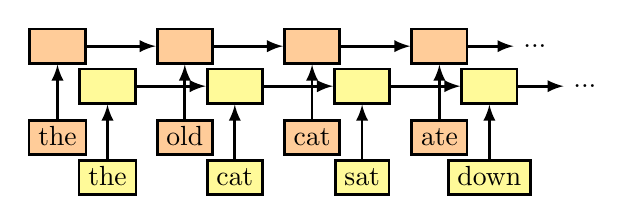
\begin{tikzpicture}
    \tikzstyle{word}=[fill=yellow!40,text height=2mm,line width=1pt,draw=black]    
    \tikzstyle{nonleaf}=[fill=yellow!40,text height=2mm,line width=1pt,draw=black] 
    \tikzstyle{alt}=[fill=orange!40]
    \pgfsetarrowsend{latex}
    \tikzstyle{fwd} = [draw=black, line width=1pt]
   
    \def\dx{23pt}
    \def\dy{11pt}
    \def\sy{7*\dy}
    \def\oxb{5.5*\dx}
    \def\by{1*\dy}
    \def\ox{0*\oxb}


    \begin{scope}[shift={(0in,0in)}, frontier/.style={distance from root=60pt}]
    
    \node[word,alt]  (w1) at (\ox+-3*\dx,\by+0*\dy) {the};
    \node[word,alt]  (w2) at (\ox+-1*\dx,\by+0*\dy) {old};
    \node[word,alt]  (w3) at (\ox+1*\dx,\by+0*\dy) {cat};
    \node[word,alt]  (w4) at (\ox+3*\dx,\by+0*\dy) {ate};

    \node[word,alt]  (n1) at (\ox+-3*\dx,\by+3*\dy) {~~~~~};
    \node[word,alt]  (n2) at (\ox+-1*\dx,\by+3*\dy) {~~~~~};
    \node[word,alt]  (n3) at (\ox+1*\dx,\by+3*\dy) {~~~~~};
    \node[word,alt]  (n4) at (\ox+3*\dx,\by+3*\dy) {~~~~~};
    \node[]  (n5) at (\ox+4.5*\dx,\by+3*\dy) {...};

   \draw [fwd] (w1) -- (n1);
   \draw [fwd] (w2) -- (n2);
   \draw [fwd] (w3) -- (n3);
   \draw [fwd] (w4) -- (n4);

   \draw [fwd] (n1) -- (n2);
   \draw [fwd] (n2) -- (n3);
   \draw [fwd] (n3) -- (n4);
   \draw [fwd] (n4) -- (n5);


    \end{scope}

    \begin{scope}[shift={(0.25in,-0.2in)}, frontier/.style={distance from root=60pt}]
    
    \node[word]  (w1) at (\ox+-3*\dx,\by+0*\dy) {the};
    \node[word]  (w2) at (\ox+-1*\dx,\by+0*\dy) {cat};
    \node[word]  (w3) at (\ox+1*\dx,\by+0*\dy) {sat};
    \node[word]  (w4) at (\ox+3*\dx,\by+0*\dy) {down};

    \node[word]  (n1) at (\ox+-3*\dx,\by+3*\dy) {~~~~~};
    \node[word]  (n2) at (\ox+-1*\dx,\by+3*\dy) {~~~~~};
    \node[word]  (n3) at (\ox+1*\dx,\by+3*\dy) {~~~~~};
    \node[word]  (n4) at (\ox+3*\dx,\by+3*\dy) {~~~~~};
    \node[]  (n5) at (\ox+4.5*\dx,\by+3*\dy) {...};


   \draw [fwd] (w1) -- (n1);
   \draw [fwd] (w2) -- (n2);
   \draw [fwd] (w3) -- (n3);
   \draw [fwd] (w4) -- (n4);

   \draw [fwd] (n1) -- (n2);
   \draw [fwd] (n2) -- (n3);
   \draw [fwd] (n3) -- (n4);
   \draw [fwd] (n4) -- (n5);

    \end{scope}

\end{tikzpicture}


\caption{\label{fig:batching:good}A conventional sequence-based RNN, instantiated for two sentences.}
\end{subfigure}

\vspace{2em}

\begin{subfigure}[t]{\columnwidth}
\begin{center}
 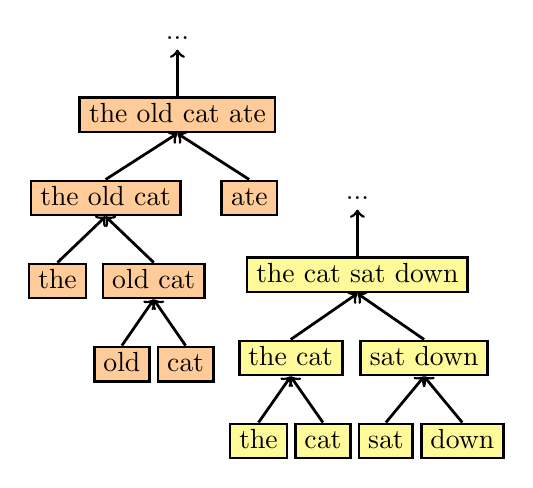
\begin{tikzpicture}
    \tikzstyle{word}=[fill=yellow!40,text height=2mm,line width=1pt,draw=black]    
    \tikzstyle{nonleaf}=[fill=yellow!40,text height=2mm,line width=1pt,draw=black]
    \tikzstyle{alt}=[fill=orange!40]    
    \pgfsetarrowsend{latex}
    \tikzset{edge from parent/.append style={<-, line width=1pt}}   

    \begin{scope}[shift={(0in,0in)}]

    \Tree [.\node[](root){...}; [.\node[nonleaf,alt](2thekittenate){the old cat ate}; [.\node[nonleaf,alt](2thekitten){the old cat}; \node[word,alt](2the){the}; [.\node[nonleaf,alt](2bigkitten){old cat}; \node[word,alt](2kitten){old}; \node[word,alt](2kitten){cat}; ] ] \node[word,alt](2ate){ate}; ] ]

    \end{scope}


    \begin{scope}[shift={(0.9in,-0.8in)}]

    \Tree [.\node[](root){...}; [.\node[nonleaf](1thecatsatdown){the cat sat down}; [.\node[nonleaf](1thecat){the cat}; \node[word](1the){the}; \node[word](1cat){cat}; ] [.\node[nonleaf](1satdown){sat down}; \node[word](1sat){sat}; \node[word](1down){down}; ] ] ]

    \end{scope}

\end{tikzpicture}
\end{center}

\caption{\label{fig:batching:bad}A conventional TreeRNN, instantiated for two sentences.}
\end{subfigure}

\caption{An illustration of two standard designs for sentence encoders. Note that the TreeRNN, unlike the sequence-based RNN, requires a substantially different connection structure for each sentence.}
\end{figure}


A wide range of current state-of-the-art models in NLP are built around neural network components that build vector representations of sentence meaning \cite{socher2011semi,sutskever2014sequence,vinyals2015neural}. This component, the sentence encoder, is generally formulated as a learned parametric function from word vectors to sentence vectors, and this function can take a range of different forms. Common sentence encoders include sequence-based recurrent neural network models (RNNs) with Long Short-Term Memory (LSTM RNNs, \citealt{hochreiter1997long}, see Figure~\ref{fig:batching:good}), which accumulate information over the sentence sequentially, convolutional neural networks over words or characters (\citealt{kalchbrenner2014convolutional}, \todo{[SB] Cite LeCun CharCNN}), which accumulate information using filters over short local sequences of words, and tree-structured recursive neural networks (TreeRNNs \citealt{goller1996learning,socher2011semi}, see Figure~\ref{fig:batching:bad}), which propagate information up a binary parse tree structure over words. Of these, it is easy to argue that the TreeRNN is the principled choice---meaning in natural language sentences is widely believed to be constructed incrementally according to a tree structure \cite{Partee84,Janssen97}, and so a model which instantiates that tree structure should have a maximally easy time learning to construct meaning.


\begin{figure*}[t]
\begin{subfigure}[t]{\textwidth}
\centering
\scalebox{0.6}{
 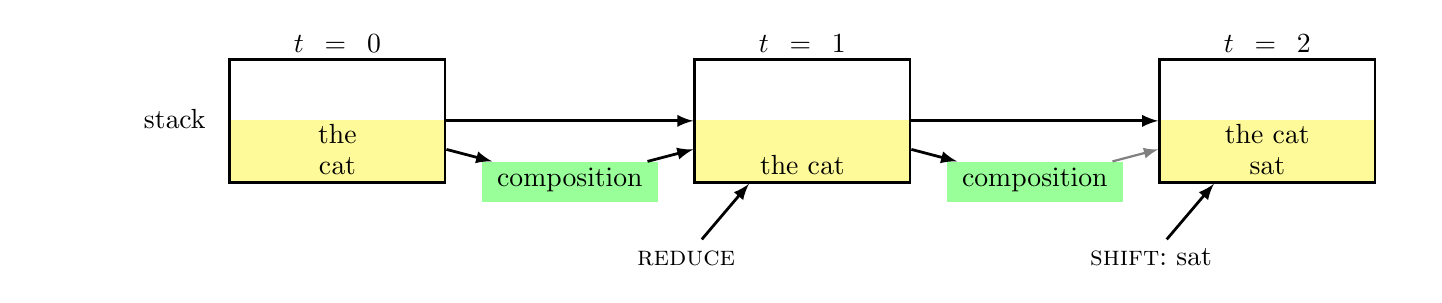
\begin{tikzpicture}
    \def\dx{21pt}
    \def\dy{11pt}
    \def\sy{13*\dy}
    \def\oxb{8*\dx}
    \def\by{1*\dy}
    \def\ox{0*\oxb}

    \tikzstyle{label}=[text width=35mm,align=center,text height=2mm]    
    \tikzstyle{word}=[text width=35mm,align=center,text height=2mm]    
    \tikzstyle{comp}=[fill=green!40,text width=20mm,align=center,text height=2mm]
    \tikzstyle{input}=[line width=1pt,text width=20mm,align=center,text height=2mm]    
    \tikzstyle{sbox}=[line width=1pt,draw=black,text width=25mm,align=center,text height=13.3mm]
    \tikzstyle{bbox}=[line width=1pt,draw=black,text width=25mm,align=center,text height=6.5mm]
    \tikzstyle{focus1}=[fill=yellow!80,opacity=0.5,text width=25mm,align=center,text height=2mm]
    \tikzstyle{focus2}=[fill=yellow!80,opacity=0.5,text width=25mm,align=center,text height=5.5mm]
    
    \node[label]  (sl) at (\ox-0.35*\oxb+0*\dx,\sy+0.5*\dy) {stack};
    
    \node[label]  (1l) at (\ox+0*\dx,\sy+3*\dy) {$t=0$};
    
    \node[focus2] (0sb) at  (\ox+0*\dx,\sy-0.5*\dy) {};
    \node[word]  (0s1) at (\ox+0*\dx,\sy-1*\dy) {cat};
    \node[word]  (0s2) at (\ox+0*\dx,\sy+0*\dy) {the};
    \node[word]  (0s3) at (\ox+0*\dx,\sy+1*\dy) {};
    \node[sbox] (0sb) at  (\ox+0*\dx,\sy+0.5*\dy) {};
    
    \node[comp] (0c) at  (\ox+0.5*\oxb,\sy-1.5*\dy) {composition};
    
    \node[input] (0so) at  (\ox+0.75*\oxb,9*\dy) {\reduce};
    
    \def\ox{1*\oxb}
    
    \node[label]  (1l) at (\ox+0*\dx,\sy+3*\dy) {$t=1$};
    
    \node[focus2] (1sb) at  (\ox+0*\dx,\sy-0.5*\dy) {};
    \node[word]  (1s1) at (\ox+0*\dx,\sy-1*\dy) {the cat};
    \node[word]  (1s2) at (\ox+0*\dx,\sy+0*\dy) {};
    \node[word]  (1s3) at (\ox+0*\dx,\sy+1*\dy) {};
    \node[sbox] (1sb) at  (\ox+0*\dx,\sy+0.5*\dy) {};
    
    \node[comp] (1c) at  (\ox+0.5*\oxb,\sy-1.5*\dy) {composition};
    
    \node[input] (1so) at  (\ox+0.75*\oxb,9*\dy) {\shift:~sat};
     
    \def\ox{2*\oxb}

    \node[label]  (1l) at (\ox+0*\dx,\sy+3*\dy) {$t=2$};

    \node[focus2] (2sb) at  (\ox+0*\dx,\sy-0.5*\dy) {};
    \node[word]  (2s1) at (\ox+0*\dx,\sy-1*\dy) {sat};
    \node[word]  (2s2) at (\ox+0*\dx,\sy+0*\dy) {the cat};
    \node[word]  (2s3) at (\ox+0*\dx,\sy+1*\dy) {};
    \node[sbox] (2sb) at  (\ox+0*\dx,\sy+0.5*\dy) {};
  
   
    \pgfsetarrowsend{latex}
    \tikzstyle{fwd} = [draw=black, line width=1pt]
    \tikzstyle{gated} = [draw=black!50, line width=0.8pt]

    \draw [fwd] (0sb) -- (0c);
    
    \draw [fwd] (0sb) -- (1sb);
    \draw [fwd] (0so) -- (1sb);
    \draw [fwd] (0c) -- (1sb);

    \draw [fwd] (1sb) -- (1c);
    
    \draw [fwd] (1sb) -- (2sb);
    \draw [fwd] (1so) -- (2sb);
    \draw [gated] (1c) -- (2sb);




  \end{tikzpicture}}
  
 \caption{\label{fig:model:0}The Model 0 network unrolled for two transitions on the input \word{the cat sat down}. The operations at the bottom of the figure are given as inputs to the models, as is the start state of the stack at $t=0$.}
  
\end{subfigure}\\\\\\
\begin{subfigure}[t]{\textwidth}
\centering
\scalebox{0.6}{
 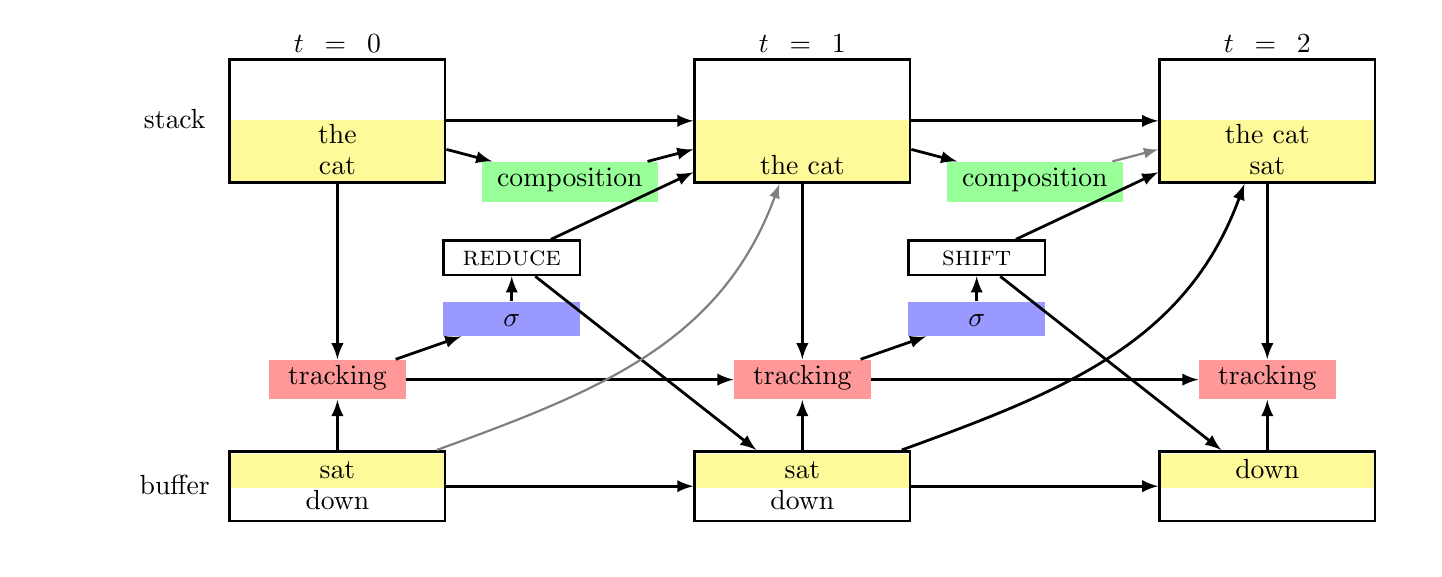
\begin{tikzpicture}
    \def\dx{21pt}
    \def\dy{11pt}
    \def\sy{13*\dy}
    \def\oxb{8*\dx}
    \def\by{1*\dy}
    \def\ox{0*\oxb}

    \tikzstyle{label}=[text width=35mm,align=center,text height=2mm]    
    \tikzstyle{word}=[text width=35mm,align=center,text height=2mm]    
    \tikzstyle{tracker}=[fill=red!40,text width=15mm,align=center,text height=2mm]
    \tikzstyle{softmax}=[fill=blue!40,text width=15mm,align=center,text height=2mm]
    \tikzstyle{comp}=[fill=green!40,text width=20mm,align=center,text height=2mm]
    \tikzstyle{result}=[line width=1pt,draw=black,text width=15mm,align=center,text height=2mm]    
    \tikzstyle{sbox}=[line width=1pt,draw=black,text width=25mm,align=center,text height=13.3mm]
    \tikzstyle{bbox}=[line width=1pt,draw=black,text width=25mm,align=center,text height=6.5mm]
    \tikzstyle{focus1}=[fill=yellow!80,opacity=0.5,text width=25mm,align=center,text height=2mm]
    \tikzstyle{focus2}=[fill=yellow!80,opacity=0.5,text width=25mm,align=center,text height=5.5mm]

    \node[label]  (sl) at (\ox-0.35*\oxb+0*\dx,\by+0.5*\dy) {buffer};

    \node[label]  (1l) at (\ox+0*\dx,\sy+3*\dy) {$t=0$};

    \node[focus1] (0bb) at  (\ox+0*\dx,2*\dy) {};
    \node[word]  (0b3) at (\ox+0*\dx,\by-1*\dy) {};
    \node[word]  (0b2) at (\ox+0*\dx,\by+0*\dy) {down};
    \node[word]  (0b1) at (\ox+0*\dx,\by+1*\dy) {sat};
    \node[bbox] (0bb) at  (\ox+0*\dx,\by+0.5*\dy) {};
    
    \node[label]  (sl) at (\ox-0.35*\oxb+0*\dx,\sy+0.5*\dy) {stack};
    
    \node[focus2] (0sb) at  (\ox+0*\dx,\sy-0.5*\dy) {};
    \node[word]  (0s1) at (\ox+0*\dx,\sy-1*\dy) {cat};
    \node[word]  (0s2) at (\ox+0*\dx,\sy+0*\dy) {the};
    \node[word]  (0s3) at (\ox+0*\dx,\sy+1*\dy) {};
    \node[sbox] (0sb) at  (\ox+0*\dx,\sy+0.5*\dy) {};
    
    \node[comp] (0c) at  (\ox+0.5*\oxb,\sy-1.5*\dy) {composition};
    
    \node[tracker] (0t) at  (\ox+0*\dx,5*\dy) {tracking};
    \node[softmax] (0sm) at  (\ox+3*\dx,7*\dy) {$\sigma$};
    \node[result] (0so) at  (\ox+3*\dx,9*\dy) {\reduce};
    
    \def\ox{1*\oxb}

    \node[label]  (1l) at (\ox+0*\dx,\sy+3*\dy) {$t=1$};

    \node[focus1] (1bb) at  (\ox+0*\dx,2*\dy) {};
    \node[word]  (1b3) at (\ox+0*\dx,\by-1*\dy) {};
    \node[word]  (1b2) at (\ox+0*\dx,\by+0*\dy) {down};
    \node[word]  (1b1) at (\ox+0*\dx,\by+1*\dy) {sat};
    \node[bbox] (1bb) at  (\ox+0*\dx,\by+0.5*\dy) {};
    
    \node[focus2] (1sb) at  (\ox+0*\dx,\sy-0.5*\dy) {};
    \node[word]  (1s1) at (\ox+0*\dx,\sy-1*\dy) {the cat};
    \node[word]  (1s2) at (\ox+0*\dx,\sy+0*\dy) {};
    \node[word]  (1s3) at (\ox+0*\dx,\sy+1*\dy) {};
    \node[sbox] (1sb) at  (\ox+0*\dx,\sy+0.5*\dy) {};
    
    \node[comp] (1c) at  (\ox+0.5*\oxb,\sy-1.5*\dy) {composition};
    
    \node[tracker] (1t) at  (\ox+0*\dx,5*\dy) {tracking};
    \node[softmax] (1sm) at  (\ox+3*\dx,7*\dy) {$\sigma$};
    \node[result] (1so) at  (\ox+3*\dx,9*\dy) {\shift};
     
    \def\ox{2*\oxb}

    \node[label]  (1l) at (\ox+0*\dx,\sy+3*\dy) {$t=2$};

    \node[focus1] (2bb) at  (\ox+0*\dx,2*\dy) {};
    \node[word]  (2b3) at (\ox+0*\dx,\by-1*\dy) {};
    \node[word]  (2b2) at (\ox+0*\dx,\by+0*\dy) {};
    \node[word]  (2b1) at (\ox+0*\dx,\by+1*\dy) {down};
    \node[bbox] (2bb) at  (\ox+0*\dx,\by+0.5*\dy) {};
    
    \node[focus2] (2sb) at  (\ox+0*\dx,\sy-0.5*\dy) {};
    \node[word]  (2s1) at (\ox+0*\dx,\sy-1*\dy) {sat};
    \node[word]  (2s2) at (\ox+0*\dx,\sy+0*\dy) {the cat};
    \node[word]  (2s3) at (\ox+0*\dx,\sy+1*\dy) {};
    \node[sbox] (2sb) at  (\ox+0*\dx,\sy+0.5*\dy) {};
   
    \node[tracker] (2t) at  (\ox+0*\dx,5*\dy) {tracking};

    
    \pgfsetarrowsend{latex}
    \tikzstyle{fwd} = [draw=black, line width=1pt]
    \tikzstyle{gated} = [draw=black!50, line width=0.8pt]

    \draw [fwd] (0sb) -- (0t);
    \draw [fwd] (0bb) -- (0t);
    \draw [fwd] (0t) -- (0sm);
    \draw [fwd] (0sm) -- (0so);
    \draw [fwd] (0sb) -- (0c);
    
    \draw [fwd] (0t) -- (1t);
    \draw [fwd] (0sb) -- (1sb);
    \draw [fwd] (0bb) -- (1bb);
    \draw [fwd] (0so) -- (1sb);
    \draw [fwd] (0so) -- (1bb);
    \draw [gated] (0bb) to[out=20,in=-110] (1sb);
    \draw [fwd] (0c) -- (1sb);

    \draw [fwd] (1sb) -- (1t);
    \draw [fwd] (1bb) -- (1t);
    \draw [fwd] (1t) -- (1sm);
    \draw [fwd] (1sm) -- (1so);
    \draw [fwd] (1sb) -- (1c);
    
    \draw [fwd] (1t) -- (2t);
    \draw [fwd] (1sb) -- (2sb);
    \draw [fwd] (1bb) -- (2bb);
    \draw [fwd] (1so) -- (2sb);
    \draw [fwd] (1so) -- (2bb);
    \draw [fwd] (1bb) to[out=20,in=-110] (2sb);
    \draw [gated] (1c) -- (2sb);

    \draw [fwd] (2sb) -- (2t);
    \draw [fwd] (2bb) -- (2t);


  \end{tikzpicture}}
  
 \caption{The Model 1/2 network unrolled for two transitions on the input \word{the cat sat down}. The start state of the stack and buffer at the initial step $t=0$ are the sole inputs to the model.}\label{fig:model:1d}
  
\end{subfigure}\\\\\\
\begin{subfigure}[t]{\textwidth}
\centering
\scalebox{0.6}{
 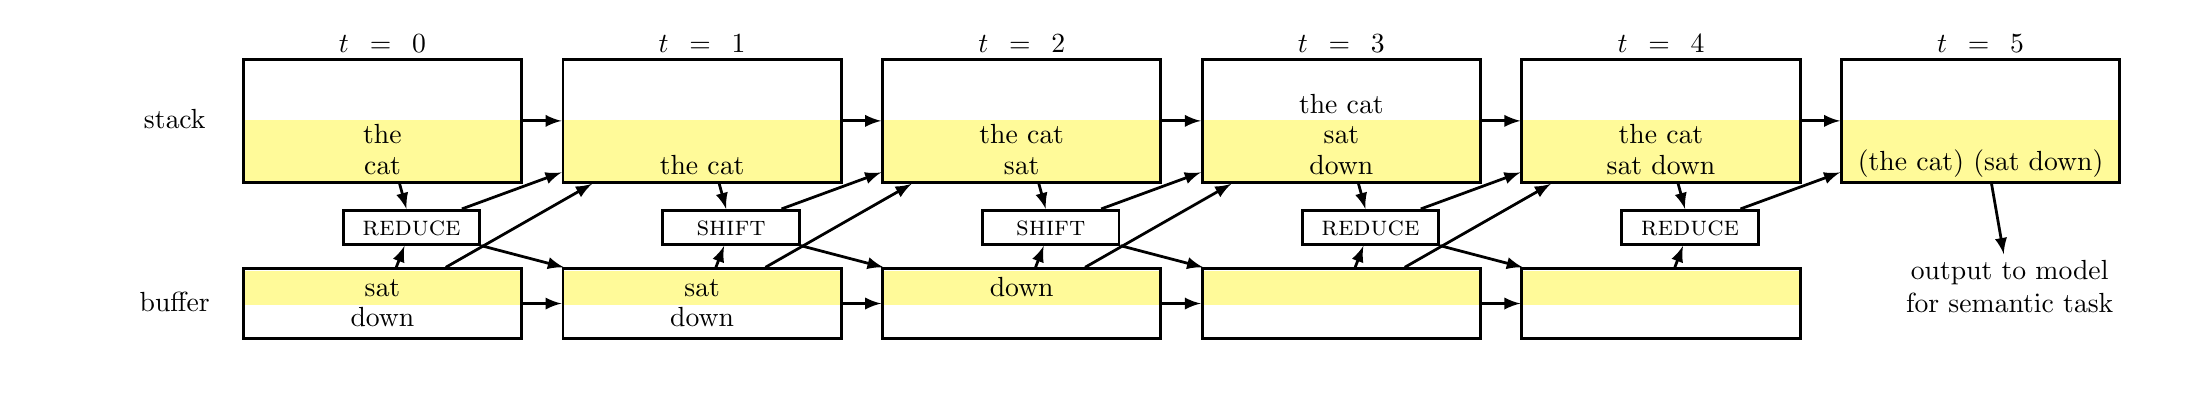
\begin{tikzpicture}
    \def\dx{21pt}
    \def\dy{11pt}
    \def\sy{7*\dy}
    \def\oxb{5.5*\dx}
    \def\by{1*\dy}
    \def\ox{0*\oxb}

    \tikzstyle{label}=[text width=35mm,align=center,text height=2mm]    
    \tikzstyle{word}=[text width=35mm,align=center,text height=2mm]    
    \tikzstyle{tracker}=[fill=red!40,text width=15mm,align=center,text height=2mm]
    \tikzstyle{softmax}=[text width=40mm,align=center,text height=2mm]
    \tikzstyle{comp}=[fill=green!40,text width=20mm,align=center,text height=2mm]
    \tikzstyle{result}=[line width=1pt,draw=black,text width=15mm,align=center,text height=2mm]    
    \tikzstyle{sbox}=[line width=1pt,draw=black,text width=33mm,align=center,text height=13.3mm]
    \tikzstyle{bbox}=[line width=1pt,draw=black,text width=33mm,align=center,text height=6.5mm]
    \tikzstyle{focus1}=[fill=yellow!80,opacity=0.5,text width=33mm,align=center,text height=2mm]
    \tikzstyle{focus2}=[fill=yellow!80,opacity=0.5,text width=33mm,align=center,text height=5.5mm]

    \def\ox{0*\oxb}
    
    \node[label]  (1l) at (\ox+0*\dx,\sy+3*\dy) {$t=0$};
    
    \node[label]  (sl) at (\ox-0.65*\oxb+0*\dx,\by+0.5*\dy) {buffer};
    
    \node[focus1] (1bb) at  (\ox+0*\dx,2*\dy) {};
    \node[word]  (1b3) at (\ox+0*\dx,\by-1*\dy) {};
    \node[word]  (1b2) at (\ox+0*\dx,\by+0*\dy) {down};
    \node[word]  (1b1) at (\ox+0*\dx,\by+1*\dy) {sat};
    \node[bbox] (1bb) at  (\ox+0*\dx,\by+0.5*\dy) {};
    
    \node[label]  (sl) at (\ox-0.65*\oxb+0*\dx,\sy+0.5*\dy) {stack};
    
    \node[focus2] (1sb) at  (\ox+0*\dx,\sy-0.5*\dy) {};
    \node[word]  (1s1) at (\ox+0*\dx,\sy-1*\dy) {cat};
    \node[word]  (1s2) at (\ox+0*\dx,\sy+0*\dy) {the};
    \node[word]  (1s3) at (\ox+0*\dx,\sy+1*\dy) {};
    \node[sbox] (1sb) at  (\ox+0*\dx,\sy+0.5*\dy) {};
    
    \node[result] (1so) at  (\ox+0.5*\dx,4*\dy) {\reduce};
              
    \def\ox{1*\oxb}
   
    \node[label]  (1l) at (\ox+0*\dx,\sy+3*\dy) {$t=1$};
    
    \node[focus1] (2bb) at  (\ox+0*\dx,2*\dy) {};
    \node[word]  (2b3) at (\ox+0*\dx,\by-1*\dy) {};
    \node[word]  (2b2) at (\ox+0*\dx,\by+0*\dy) {down};
    \node[word]  (2b1) at (\ox+0*\dx,\by+1*\dy) {sat};
    \node[bbox] (2bb) at  (\ox+0*\dx,\by+0.5*\dy) {};
    
    \node[focus2] (2sb) at  (\ox+0*\dx,\sy-0.5*\dy) {};
    \node[word]  (2s1) at (\ox+0*\dx,\sy-1*\dy) {the cat};
    \node[word]  (2s2) at (\ox+0*\dx,\sy+0*\dy) {};
    \node[word]  (2s3) at (\ox+0*\dx,\sy+1*\dy) {};
    \node[sbox] (2sb) at  (\ox+0*\dx,\sy+0.5*\dy) {};
    
    \node[result] (2so) at  (\ox+0.5*\dx,4*\dy) {\shift};
             
    \def\ox{2*\oxb}
    
    \node[label]  (1l) at (\ox+0*\dx,\sy+3*\dy) {$t=2$};
    
    \node[focus1] (3bb) at  (\ox+0*\dx,2*\dy) {};
    \node[word]  (3b3) at (\ox+0*\dx,\by-1*\dy) {};
    \node[word]  (3b2) at (\ox+0*\dx,\by+0*\dy) {};
    \node[word]  (3b1) at (\ox+0*\dx,\by+1*\dy) {down};
    \node[bbox] (3bb) at  (\ox+0*\dx,\by+0.5*\dy) {};
    
    \node[focus2] (3sb) at  (\ox+0*\dx,\sy-0.5*\dy) {};
    \node[word]  (3s1) at (\ox+0*\dx,\sy-1*\dy) {sat};
    \node[word]  (3s2) at (\ox+0*\dx,\sy+0*\dy) {the cat};
    \node[word]  (3s3) at (\ox+0*\dx,\sy+1*\dy) {};
    \node[sbox] (3sb) at  (\ox+0*\dx,\sy+0.5*\dy) {};
    
    \node[result] (3so) at  (\ox+0.5*\dx,4*\dy) {\shift};

    \def\ox{3*\oxb}
    
    \node[label]  (1l) at (\ox+0*\dx,\sy+3*\dy) {$t=3$};
        
    \node[focus1] (4bb) at  (\ox+0*\dx,2*\dy) {};
    \node[word]  (4b3) at (\ox+0*\dx,\by-1*\dy) {};
    \node[word]  (4b2) at (\ox+0*\dx,\by+0*\dy) {};
    \node[word]  (4b1) at (\ox+0*\dx,\by+1*\dy) {};
    \node[bbox] (4bb) at  (\ox+0*\dx,\by+0.5*\dy) {};
    
    \node[focus2] (4sb) at  (\ox+0*\dx,\sy-0.5*\dy) {};
    \node[word]  (4s1) at (\ox+0*\dx,\sy-1*\dy) {down};
    \node[word]  (4s2) at (\ox+0*\dx,\sy+0*\dy) {sat};
    \node[word]  (4s3) at (\ox+0*\dx,\sy+1*\dy) {the cat};
    \node[sbox] (4sb) at  (\ox+0*\dx,\sy+0.5*\dy) {};
    
    \node[result] (4so) at  (\ox+0.5*\dx,4*\dy) {\reduce};
                  
    \def\ox{4*\oxb}
    
    \node[label]  (1l) at (\ox+0*\dx,\sy+3*\dy) {$t=4$};
    
    \node[focus1] (5bb) at  (\ox+0*\dx,2*\dy) {};
    \node[word]  (5b3) at (\ox+0*\dx,\by-1*\dy) {};
    \node[word]  (5b2) at (\ox+0*\dx,\by+0*\dy) {};
    \node[word]  (5b1) at (\ox+0*\dx,\by+1*\dy) {};
    \node[bbox] (5bb) at  (\ox+0*\dx,\by+0.5*\dy) {};
    
    \node[focus2] (5sb) at  (\ox+0*\dx,\sy-0.5*\dy) {};
    \node[word]  (5s1) at (\ox+0*\dx,\sy-1*\dy) {sat down};
    \node[word]  (5s2) at (\ox+0*\dx,\sy+0*\dy) {the cat};
    \node[word]  (5s3) at (\ox+0*\dx,\sy+1*\dy) {};
    \node[sbox] (5sb) at  (\ox+0*\dx,\sy+0.5*\dy) {};
    
    \node[result] (5so) at  (\ox+0.5*\dx,4*\dy) {\reduce};
    
    \def\ox{5*\oxb}

    \node[label]  (1l) at (\ox+0*\dx,\sy+3*\dy) {$t=5$};

    \node[focus2] (6sb) at  (\ox+0*\dx,\sy-0.5*\dy) {};
    \node[word]  (6s1) at (\ox+0*\dx,\sy-1*\dy) {(the cat) (sat down)};
    \node[word]  (6s2) at (\ox+0*\dx,\sy+0*\dy) {};
    \node[word]  (6s3) at (\ox+0*\dx,\sy+1*\dy) {};
    \node[sbox] (6sb) at  (\ox+0*\dx,\sy+0.5*\dy) {};

    \node[softmax] (6sm) at  (\ox+0.5*\dx,2*\dy) {output to model for semantic task};
                   
    \pgfsetarrowsend{latex}
    \tikzstyle{fwd} = [draw=black, line width=1pt]

   \draw [fwd] (1sb) -- (1so);
   \draw [fwd] (1bb) -- (1so);

    \draw [fwd] (1sb) -- (2sb);
    \draw [fwd] (1bb) -- (2bb);
    \draw [fwd] (1so) -- (2sb);
    \draw [fwd] (1so) -- (2bb);
    \draw [fwd] (1bb) -- (2sb);

   \draw [fwd] (2sb) -- (2so);
   \draw [fwd] (2bb) -- (2so);

    \draw [fwd] (2sb) -- (3sb);
    \draw [fwd] (2bb) -- (3bb);
    \draw [fwd] (2so) -- (3sb);
    \draw [fwd] (2so) -- (3bb);
    \draw [fwd] (2bb) -- (3sb);

   \draw [fwd] (3sb) -- (3so);
   \draw [fwd] (3bb) -- (3so);

    \draw [fwd] (3sb) -- (4sb);
    \draw [fwd] (3bb) -- (4bb);
    \draw [fwd] (3so) -- (4sb);
    \draw [fwd] (3so) -- (4bb);
    \draw [fwd] (3bb) -- (4sb);

   \draw [fwd] (4sb) -- (4so);
   \draw [fwd] (4bb) -- (4so);

    \draw [fwd] (4sb) -- (5sb);
    \draw [fwd] (4bb) -- (5bb);
    \draw [fwd] (4so) -- (5sb);
    \draw [fwd] (4so) -- (5bb);
    \draw [fwd] (4bb) -- (5sb);

   \draw [fwd] (5sb) -- (5so);
   \draw [fwd] (5bb) -- (5so);

    \draw [fwd] (5sb) -- (6sb);
    \draw [fwd] (5so) -- (6sb);

   \draw [fwd] (6sb) -- (6sm);

  \end{tikzpicture}}
  
 \caption{The fully unrolled Model 1/2 network for \word{the cat sat down} with some layers omitted for clarity.}\label{fig:model:1b}  
\end{subfigure}
\caption{\label{m1-views}Two views of Models 1 and 2 (which use equivalent model graphs). In both views, the lower boxes represent the input buffer, and the upper boxes represent the stack. Yellow highlighting indicates which portions of these data structures are visible to the tracking LSTM and to the composition function. Thin gray arrows indicate connections which are blocked by a gating function, and so contribute no information.}
\end{figure*}

TreeRNNs have shown promise, but they have largely been overlooked in favor of sequence-based RNNs for practical reasons. Batched computation---performing synchronized computation across many examples at once---is a crucial enabling technology in allowing neural networks to be trained efficiently on large datasets (\question{What, if anything, can we cite here?}). Batching yields order-of-magnitude improvements in standard CPU implementations of neural network models, and substantial additional gains on GPUs. TreeRNNs build the parse structure of each sentence they process into the structure of the network itself, forcing the model to perform a different sequence of computations for each sentence, and thereby requiring that each sentence be processed one-by-one, making batched computation impossible in standard implementations. One aim of this paper is to restructure the computations involved in a TreeRNN in order to enable batching and make these large-scale evaluations possible.  In addition to their slow speed, TreeRNNs have an additional feature that makes them impractical in many settings: they can only operate on sentences that have already been processed by a syntactic parser, which slows and complicates the implementation of these models for most applications. This paper additionally aims to integrate parsing into TreeRNN processing to circumvent this issue.

In spite of the unwieldiness of current standard TreeRNNs, there is still value in the idea of using syntactic parse trees to guide the construction of meaning in neural network models. Tree-structured models have shown substantial performance gains on some smaller-scale NLP tasks \cite{tai2015improved,li2015tree}, and their theoretical foundations are strong. Tree-structured compositionality is a property of natural language, and simpler sequence-based RNNs have a difficult time exploiting this property---while sequence-based models should, theoretically, be able to learn to simulate tree-structured composition, this behavior does not emerge in practice on reasonably-sized tasks \cite{bowman2015trees}. 

In this paper, we introduce the Stack-augmented Parser-Interpreter Neural Network, or SPINN. The SPINN executes tree-structured computations in a linearized sequence, and can incorporate a neural network parser that determines the overall tree structure on-the-fly. This design improves upon the previous TreeRNN approach to compositionality in three ways:
\begin{itemize}
\item At test time, it can simultaneously parse and interpret unparsed sentences, removing the dependence on an external parser.
\item It supports batched computation for both parsed and unparsed sentences, supporting dramatic speedups over standard TreeRNNs.
\item It supports a novel tree-sequence hybrid mechanism for handling local context in sentence interpretation that yields substantial gains in accuracy over either pure sequence-based models or pure tree-based models.
\end{itemize}

\section{The shift-reduce sentence model}

\subsection{Shift-reduce parsing}

The SPINN is inspired by the shift-reduce parsing formalism \cite{aho1986compilers}, which builds a tree structure over a sequence (e.g. a natural language sentence) by a single left-to-right scan over the tokens of the sequence. Shift-reduce parsing has been successfully applied in algorithms for natural language parsing \cite{nivre2003efficient}.

A shift-reduce parser accepts a sequence of input tokens $\mathbf x = (x_1, \dots, x_N)$ and transitions $\mathbf t = (t_1, \dots, t_T)$. It reads left-to-right over the input transition sequence, combining the input tokens $\mathbf x$ incrementally into a tree structure. (For a binary-branching tree structure, this requires $T = 2N - 1$ operations.)

The parser uses two auxiliary data structures, a stack $S$ of partially completed subtrees and a buffer $B$ of tokens yet to be parsed. We initialize the parser with an empty stack and with a buffer containing all the sentence tokens $\mathbf x$. Let $\langle S, B \rangle = \langle \emptyset, \mathbf x \rangle$ denote this starting state. We next proceed through the transition sequence, where each transition $t_i$ selects one of the two following operations. Below $\mid$ denotes an infix \textit{cons} function.
\begin{description}
  \item[\shift:] $\langle S, x \mid B \rangle \to \langle x \mid S, B \rangle$. This operation pops an element from the buffer and pushes it onto the top of the stack.
  \item[\reduce:] $\langle x \mid y \mid S, B \rangle \to \langle (x, y) \mid S, B \rangle$. This operation pops the top two elements from the stack, merges them into a binary tree with children $(x, y)$, and pushes the result back onto the stack.
\end{description}

\subsection{Composition and representation}

The core SPINN model implements a sequential shift-reduce parser which operates over sentences. It is designed to produce a vector representation of the sentence as output (as opposed to a tree). This is accomplished by the following modifications to the shift-reduce algorithm:
\begin{itemize}
\item The intermediate representations in the parser, including the representations of partial tree structures on the stack, are fixed-length vectors.
\item The \reduce~operation combines two such representations of trees on the stack into a larger tree using a neural network.
\end{itemize}

This subsection describes the core functions and representations of the SPINN. We begin with the most basic model, SPINN-NP (for \textit{no parser}), which processes input sentences with gold parses provided by some external parser.

\paragraph{The buffer and word representations}

We draw our word representations from the standard 300-dimensional vector package provided with GloVe \cite{pennington2014glove}. We do not update these vectors during training. Instead, we use a learned linear transformation to transform the representation of each input word $\vec{x}$ into a pair of vectors that can be used as inputs to a TreeLSTM composition function:

\begin{equation}
\colvec{2}
    {\vec{h}}
    {\vec{c}}
= W_{\text{wd}} \vec{x}
\end{equation}


\paragraph{The stack and buffer}

In a SPINN, each row of the stack contains a pair of vectors $(h, c)$, which together represent some node in the parse tree of the sentence. Since the \shift~operation simply copies entries from the buffer onto the stack, this means that the word representations in the buffer also have two parts, $h$ and $c$. 

\paragraph{The composition function}
When a \reduce~operation is performed, vector representations of two tree nodes are popped off of the head of the stack and fed into a {\ii composition function}, which is a neural network function that produces a representation for a new tree node that is the parent of the two popped nodes. This new node is then pushed on to the stack.

Our composition function is based on the TreeLSTM of \citealt{tai2015improved}. The TreeLSTM generalizes the LSTM neural network layer \cite{hochreiter1997long} to tree- rather than sequence-based inputs, and it shares with that older design the idea of representing intermediate states in a computation using a two-part vector representation containing an $\vec{h}$ vector and a $\vec{c}$ vector, where the latter is meant to serve as a slower-changing long-term memory.  It is formulated as:

\begin{gather}
\colvec{4}
    {\vec{i}}
    {\vec{f}_l}
    {\vec{f}_r}
    {\vec{o}}
= \sigma\left(
W_{\text{iffo}}
\colvec{3}
    {\vec{h}_s^1}
    {\vec{h}_s^2}
    {\vec{e}}
\right)
\\
\vec{g}
= \tanh\left(
W_{g}
\colvec{3}
    {\vec{h}_s^1}
    {\vec{h}_s^2}
    {\vec{e}}
\right)
\\
\vec{c} = \vec{f}_l \odot \vec{c}_s^{\,2} + \vec{f}_r \odot \vec{c}_s^{\,1} + \vec{i} \odot \vec{g}  
\\
\vec{h} = \vec{o} \odot \vec{c}
\end{gather}

The results of this function are the pair $\langle\vec{h}, \vec{c}\rangle$, which are placed back on the stack. The two input tree nodes popped off the stack are represented as the pairs $\langle\vec{h}^1_s, \vec{c}^{\,1}_s\rangle$ and $\langle\vec{h}^2_s, \vec{c}^{\,2}_s\rangle$. In addition, $\vec{e}$ is an optional input argument which is either the empty vector $[]$ or a vector from an external source like the tracking LSTM (see below). $\odot$ denotes the elementwise product. Each vector-valued variable listed here is of dimension $D$, except $\vec{e}$, which is of dimensions $D_t$, which can be chosen independently.

\paragraph{Creating a sentence pair classifier}

This paper presents the transition-based sentence model within the context of \textit{natural language inference} (also known as \textit{recognizing textual entailment}), a sentence pair classification task. To classify a sentence pair, a feature vector is first constructed. This feature vector is based on the final representations of each of the two sentences---the representations that appear at the head of the stack for each sentence after the final transition. In particular, the $\vec{h}$ portions of these representations are used. The final feature vector consists of the concatenation of these two vectors, $\vec{x}_{\text{premise}}$ and $\vec{x}_{\text{hypothesis}}$, their difference, and their elementwise product:

\begin{equation}
\vec{x}_{classifier} = 
\colvec{4}
    {\vec{h}_{\text{premise}}}
    {\vec{h}_{\text{hypothesis}}}
    {\vec{h}_{\text{premise}} - \vec{h}_{\text{hypothesis}}}
    {\vec{h}_{\text{premise}} \odot \vec{h}_{\text{hypothesis}}}
\end{equation}

This feature vector is then passed to a series of two (\todo{Update w/ final number}) ReLU neural network layers (following \citealt{snli:emnlp2015}), then passed into a linear transformation, and then finally passed to a softmax layer, which yields a distribution among the three labels.

\subsection{Tracking left context with an auxiliary LSTM}

While it is possible to use the model that we have described thus far as a sentence encoder, at least when an external parser is available to supply \shift~and \reduce~instructions (and we do evaluate such a model), our full model includes an additional component: the tracking LSTM. The tracking LSTM is a simple low-dimensional sequence-based LSTM RNN that operates in tandem with the model, taking inputs from the buffer and stack at each step. It is meant to maintain a low-resolution summary of the portion of the sentence that has been processed so far, and it is used for two purposes: it supplies feature representations to the transition decision function, which is what allows the model to stand alone as a parser, and it additionally supplies a secondary input to the composition function, allowing context information to leak into the construction of sentence meaning, and forming what is effectively a tree-sequence hybrid model.

Technically, the tracking LSTM takes three vectors as inputs at each step: the top element of the buffer $\vec{h}_b^1$, which would be moved in a \shift~operation, and the two two elements of the stack $\vec{h}_s^1$ and $\vec{h}_s^2$ which would be composed in a \reduce~operation. Its output hidden state at each step is used as the external input to the TreeLSTM composition function for that step and as the sole input to the transition prediction function.

\paragraph{Tracking left context for parsing} The decision function which determines which transitions (and thereby, which parses) the SPINN will use needs to take as its input some representation of the current state of the model. Because the tracking LSTM directly takes the buffer top as input, it can directly inform that function of what word is under consideration for a possible \shift. Because the tracking LSTM sees the top of the stack at every step, and information only enters the stack by being at the top at some step, the tracking LSTM is able to supply that function with a summary of the state of the stack without having to iterate over the full stack at each step.

\paragraph{Tracking left context for interpretation} Lexical ambiguity is omnipresent in natural language. Most words have multiple senses or meanings, and it is generally necessary to use the context in which a word occurs to determine which of its senses or meanings is meant in a given sentence. Simpler sequence-based sentence encoding models like the standard LSTM RNN have an advantage here: when a sequence-based model first processes a word (first incorporates it into a partial sentence representation), the model has access to a state vector that summarizes all of the words to the left of the current word, and that state vector can serve as a crude but effective form of context to help with disambiguation. In contrast, when standard tree-structured models first process a word, they only have access to the constituent that the word is merging with, which is strictly less than the sequence model has access to, and is often just a single additional word. Feeding a context representation from the tracking LSTM into the composition function is a simple and efficient way to mitigate this disadvantage of tree-structured models.

\todo{[JG] Include figure of post-order traversal sequence made by the tracking LSTM?}
\todo{[SB] Say more about joint learning of phrase representations for the two objectives.}

\paragraph{The full objective function} \todo{[SB] Fill out. In short, there are two weighted terms in the objective: a semantic term and a syntactic term.}

\subsection{Parsing: Predicting transitions from the tracking state}

The model described so far is the SPINN-NP model, which uses sequences of \shift~and \reduce~operations from an external parser. To build the fully independent SPINN model, we simply add a single-layer neural network classifier that chooses which operation to perform at each step using the state of the tracking LSTM:
\begin{equation}
\vec{p}_{trans} = \text{softmax}(W_{trans}\vec{h}_{track})
\end{equation}

The resulting vector $\vec{p}_{trans}$ is a probability distribution over parsing decisions (i.e., predicting whether to \shift~or \reduce~at the current timestep). In the full SPINN model, we follow whichever transition has a higher predicted probability in this distribution. This prediction module is trained to mimic the decisions of an external parser. In particular, we use the transition sequences corresponding to the constituency parses included in the SNLI corpus. The classifier is trained using a cross-entropy objective:
\begin{equation}
  L_{trans} = - \log \vec{p}_{trans}[t^*]
\end{equation}
where $t^*$ is the correct transition specified by the gold parse, and $\vec{p}[\cdot]$ represents vector indexing.

At training time, the model follows the transitions corresponding to the gold parse. At test time, a transition is chosen at each step by taking a hard max over the output of this function. We did not find the technique of scheduled sampling \cite{bengio2015scheduled}, or allowing the model to use its own transition decisions in some instances at training time, to be helpful.

\subsection{Implementing the transition-based sentence model}

\paragraph{The size of the stack}
The size of the stack should be $N$ for sentences of $N$ words, in case the first \reduce~operation merges the final two words. The size of the buffer should be $N$.

\paragraph{Converting parses to transition sequences}

For Models 0--3, all training data must be parsed in advance into an unlabeled binary constituency tree. In addition, Model 0 requires that  parses be available at test time as well. For both SST and SNLI we use the parses included with the corpus distributions whenever parses are needed. 

For model 0, training data can be prepared by linearizing the provided parse, then deleting left brackets and replacing right brackets with \reduce~instructions. That is demonstrated here with the example sentence \ii{the cat sat down}:

\begin{quote}\small
( ( the cat ) ( sat down ) )$\Rightarrow$\\
the cat \reduce~sat down \reduce~\reduce
\end{quote}

The input for models 1--4 is simply the word sequence from the parse, with the first two words moved into the stack. The syntactic supervision labels for models 1--3 are simply a binarized version of the Model 0 inputs, with the first two tokens (which are necessarily \shift~\shift) omitted: 

\begin{quote}\small
( ( the cat ) ( sat down ) )$\Rightarrow$ \\
stack: $\langle$the, cat$\rangle$\\
buffer: $\langle$sat, down$\rangle$\\
ops: \reduce~\shift~\shift~\reduce~\reduce
\end{quote}

\paragraph{Handling variable sentence lengths}

To efficiently implement batched computation, we must stipulate a fixed number of transitions (50) that the model can perform before producing an output. Sentences whose transition sequences are shorter than this length are padded, and sentences whose transition sequences are longer than this length are cropped. 

Padding, if done properly, should not impact the output of the model significantly:\footnote{The tracking LSTM can cause a slight dependence of the final representation on unrolling length. Because of this, we always train and test the model with a fixed unrolling length.} a model with the fixed parameters should produce the same representation for a 10-word sentence whether it is unrolled for 19 transitions (the minimum to avoid cropping) or 100.

Cropping necessarily discards information, but if done properly, it is nonetheless possible to learn good representations for cropped sentences. When a transition sequence is cropped, the number of removed \shift~transitions is tracked, and an equal number of word tokens is removed from the tail (left) end of the buffer. This makes it possible for a transition sequence to begin with a \reduce~transition, or to otherwise use a \reduce~transition on a stack that does not have two elements to merge. In this instance, we simply feed the composition function one or more zero vectors, which represent nonexistent stack elements. If the composition learns to interpret these zero vectors properly, they can be taken to be unknown or incomplete nodes in an otherwise complete tree that is constructed according to the intended parse structure. \todo{[SB] Make a figure showing the results of cropping if there's room.}

\paragraph{Optimization and hyperparameters}

We use the RMSProp optimizer (\todo{[SB] Cite.}) with a tuned starting learning rate that decays by a factor of 0.75 every 10k steps. We apply both dropout \cite{srivastava2014dropout} and batch normalization \cite{2015SIoffeCSzegedy} to the word embeddings in the buffer (after the linear projection is applied) and to the feature vectors that serve as the inputs and outputs to the MLP that precedes the final entailment classifier. In addition, we apply an L2 regularization penalty to all parameters.

We used random search to tune many of the hyperparameters, including the learning rate, the dropout rate, the L2 regularization weight, the hidden dimension of the tracking LSTM and the number of layers in the MLP \todo{[SB] Report the ranges searched for each parameter and the number of runs for each results. Some of this can go in an appendix.}

We trained each model for 250k steps in each run, using a minibatch size of 32 for each step. We tracked each model's performance on the development set during training and saving parameters when this performance reached a new peak. We used early stopping, evaluating on the test set using the parameters that performed best on the development set.

\paragraph{Software infrastructure} We will make Theano code available.

\subsection{Efficient stack representation}

A naive implementation of the SPINN model would require simulating a stack of size $N$ for each input sentence. In order to update the model weights via backpropagation, we would also need to maintain all intermediate stack representations for later chain rule calculations. This implies a total space requirement of $B \times N \times T \times D$, which is prohibitively large for significant batch sizes $B$ or sentence lengths $N$. Such a naive implementation would also require duplicating a largely unchanged stack at each timestep (as \shift~and \reduce~operations only affect the top of the stack).

We designed an alternative minimal-space stack algorithm inspired by the zipper technique \cite{huet1997zipper}. For a single input sentence, we represent the stack with a single $T \times D$ matrix $S$. \todo{[JG] Either expand or remove references to batch size.} Each row $S_t$ represents the top of the actual stack at timestep $t$. We maintain a queue of backpointers onto $S$ in order to track which elements should be involved in a \reduce~operation at any given time. Algorithm~\ref{alg:thin-stack} below describes the full mechanics of a stack feedforward in this compressed representation. It operates on the compressed $T \times D$ matrix $S$ and a backpointer queue $Q$. Table~\ref{tbl:thin-stack} shows an example run of this algorithm.

\begin{algorithm}
\caption{The thin-stack algorithm}
\label{alg:thin-stack}
\begin{algorithmic}[1]
  \Function{Step}{bufferTop, op, $t$, $S$, $Q$}
    \If{op = \shift}
      \State $S$[$t$] := bufferTop
    \ElsIf{op = \reduce}
      \State right := $S$[$Q$.pop()]
      \State left := $S$[$Q$.pop()]
      \State $S$[$t$] := \Call{Compose}{left, right}
    \EndIf
    \State $Q$.push($t$)
  \EndFunction
\end{algorithmic}
\end{algorithm}

This stack representation requires substantially less space. It stores each element involved in the feedforward computation exactly once, meaning that this representation can still support efficient backpropagation. Furthermore, all of the updates to $S$ and $Q$ can be performed in-place on a GPU. These features allow this stack model to run efficiently on a GPU. We describe speed results in Section~\ref{sec:speed}.

\begin{table}
\centering
\begin{tabular}{c|cl}
  \toprule
  $t$ & $S$[$t$] & $Q_t$ \\
  \midrule
  0 & $a$ & 0 \\
  1 & $b$ & 0 1 \\
  2 & $c$ & 0 1 2 \\
  3 & $(c~b)$ & 0 3 \\
  4 & $((c~b)~a)$ & 4 \\
  \bottomrule
\end{tabular}
\caption{An example of the thin-stack algorithm computing a \shift-\shift-\shift-\reduce-\reduce~sequence on the input sentence $(a, b, c)$. $S$ is shown in the second column and may be thought of as a list of the tops of the stack at all timesteps $t$. The last two elements of $Q$ specify the rows $t$ which should be involved in a \reduce~operation at the next timestep.}
\label{tbl:thin-stack}
\end{table}

\subsection{TreeRNN-equivalence and efficiency}

In its bare form, before the addition of the tracking LSTM, the SPINN (or, SPINN-NP-NT, for \textit{no parsing, no tracking}) computes the precisely the same functions as a conventional tree-structured neural network model, and has the same learning dynamics: the representation of each sentence consists of the representation of the words, combined recursively using a TreeRNN composition function (in our case, the TreeLSTM function). While it adds no expressive power on its own, this design improves upon the standard TreeRNN implementation in three ways:

\begin{itemize}
\item It provides a straightforward strategy for implementing tree-structured composition which allows for batched computation, and provides near-optimal run times on typical computer systems. While our design includes some wasted computation induced by the full application of the composition function at every step, this is made up for by avoiding most of the (potentially expensive) scattered memory access that would be needed for batched computation strategies that more closely mimic the standard tree-based architecture.

\item It provides a simple mechanism for integrating the use of left-context into tree-structured models through the tracking LSTM, providing a fast mechanism to help these models handle lexical ambiguity.

\item By designing the model around the standard transition set used in neural network syntactic parsers, it opens the door to tight integration between parsing and sentence interpretation, including the possibility of joint learning, or even of learning a parser trained entirely on a sentence classification or interpretation objective.
\end{itemize}

\subsection{Related work: Transition-based parsing and neural networks.}

There has been a fairly long history of work on building neural-network based parsers that use the core operations and data structures from transition-based parsing \cite{henderson2004discriminative,emami2005neural,titov2010latent,buys2generative,chen2014,dyer-EtAl:2015:ACL-IJCNLP,kiperwasser2016easy}. In addition, there has been recent work \cite{zhang2016top,dyer2016rnn} proposing models designed primarily for generative language modeling tasks that use these structures as well. To our knowledge, the SPINN is the first model to use these structures for the purpose of sentence interpretation, rather than parsing or generation.

\section{Experiments}

\begin{table*}[t]
  \centering\small
  \begin{tabular}{lcccc} 
    \toprule
Model                   & Params.    & Trans. acc.  &   Train  &   Test \\
\midrule
\multicolumn{5}{c}{Previous non-NN results}\\
\midrule
Lexicalized classifier \cite{snli:emnlp2015}
                        & --                & --                    &   99.7   &   78.2      \\
\midrule
\multicolumn{5}{c}{Previous sentence encoder-based NN results}\\
\midrule
100d LSTM encoders \cite{snli:emnlp2015}
                        & 221k               & --               &   84.8   &   77.6      \\
1024d pretrained GRU encoders \cite{DBLP:journals/corr/VendrovKFU15}
                        & 15m                & --              &   98.8   &   81.4       \\
300d Tree-based CNN encoders \cite{mou2015recognizing}
                        & 3.5m                & --             &   83.4   &   82.1       \\
\midrule
\multicolumn{5}{c}{Our results}\\
\midrule
300d LSTM RNN encoders          & 3.0m                  & --                &   83.9      &   80.6       \\
\result{300d SPINN-NP-NT}   
                        & 3.4m                  & --                &   ?      &   81.9dv       \\
\result{300d SPINN-NP}
                        & 3.7m                  & --                &   ?      &   \underline{84.8dv}       \\
\result{300d SPINN }
                        & ??                  & 92.2+dv            &   ?    &   83.3+dv       \\          
% \result{300d SPINN-NP, sequence-based attn.   }     
%                         & ?                  & --                &   ?      &   86.3dv         \\
% \result{300d SPINN-NP, tree-based attn. }           
%                         & ?                  & --                &   ?      &   \textbf{?}\\
\midrule
\multicolumn{5}{c}{Other previous NN results}\\
\midrule
100d LSTM w/ word-by-word attention \cite{rocktaschel2015reasoning}
                        & 252k               & --              &   85.3   &   83.5       \\
300d mLSTM word-by-word attention model \cite{DBLP:journals/corr/WangJ15b}
                        & 1.9m               & --             &   92.0   &   86.1      \\
300d LSTMN with deep attention fusion \cite{cheng2016long}
                        & 1.4m               & --                &   92.3   &   \textbf{89.1}      \\
    \bottomrule
  \end{tabular}
  \protect\caption{\protect\label{tab:results}Results on SNLI 3-way inference classification. Params. is the approximate number of trained parameters (excluding word embeddings for models where they are trained). Trans. acc. is the model's accuracy in predicting parsing transitions. Train and test are SNLI classification accuracy.} 
\end{table*}


\subsection{Natural language inference and SNLI}

We evaluate the SPINN on the task of natural language inference (NLI), also known as recognizing textual entailment (RTE). NLI is a sentence pair classification task, in which a model reads two sentences (a premise and a hypothesis), and outputs a judgment of {\it entailment}, {\it contradiction}, or {\it neutral}, reflecting the relationship between the meanings of the two sentences, as in this example from the Stanford NLI corpus (SNLI, \citealt{snli:emnlp2015}), which we use for training and evaluation: 

\begin{quote}
Premise: {\it Girl in a red coat, blue head wrap and jeans is making a snow angel.}

Hypothesis: {\it A girl outside plays in the snow.}

Correct label: {\it entailment}
\end{quote}

Even though NLI is framed as a relatively simple three-way classification task, it is nonetheless an effective way of evaluating the ability of some model to extract broadly informative representations of sentence meaning. In order for a model to perform reliably well on NLI across a range of sentence types and text genres, it must be able to represent and reason with all of the core phenomena of natural language semantics, including quantification, coreference, scope, and several types of ambiguity.

SNLI is a corpus of 570k human-labeled pairs of scene descriptions like the one above. We use the standard train--test split and ignore unlabeled examples, which leaves about 549k examples for training, 9,842 for development, and 9,824 for testing. SNLI labels are roughly balanced, with the most frequent label, {\it entailment}, making up 34.2\% of the test set.


\subsection{Models evaluated}

We evaluate four models on the SNLI task. Each uses 300d hidden states:
\begin{itemize}
\item A baseline LSTM model (similar to that of \citealt{snli:emnlp2015}) that uses the same classifier architecture as our models, but encodes sentences using a single layer LSTM-RNN sequence model.
\item The minimal SPINN-NP-NT (\textit{no parsing, no tracking}) model, which uses transitions from an external parser, and has no tracking LSTM to inform semantic composition. This model is equivalent to a TreeLSTM \cite{tai2015improved}.
\item The SPINN-NP model, which includes a tracking LSTM which guides composition, making it a hybrid tree-sequence model.
\item The full SPINN model, which makes its own parsing decisions, and does not depend on an external parser at test time, making it slightly weaker but a practical choice in applied settings.
\end{itemize}

We compare our models against a range of baselines, including the strongest published non-neural network-based result from \cite{snli:emnlp2015}, a set of previous neural network models built around sentence encoders, and a set of models built around soft attention architectures. We should note that these attention-based models are by far the strongest published on SNLI to date, but we do not wish to compare our model with those models directly. SNLI was originally presented as an evaluation and development task for sentence encoding models, on the premise that sentence encoding models that do well on SNLI capture sentence meaning in a general sense, and are well suited to use on a range of NLP tasks. The attentional models are narrowly adapted to the sentence-pair structure of SNLI examples and cannot act as such general sentence encoders. We focus on models which do support general sentence encoding in our analysis.


\paragraph{Results} Table~\ref{tab:results} shows our results. Our primary evaluation metric for all models is three-way classification accuracy on the SNLI test set. The full SPINN model also generates parsing predictions, and we report a measure of agreement between this model's predictions and the Stanford Parser's predictions on the same data (calculated as classification accuracy over \shift~and \reduce~operations). We also report the number of trained parameters in each model and training set accuracy.

We find that the bare SPINN-NP-NT model performs relatively poorly, but that the SPINN-NP with the added tracking LSTM reaches state-of-the-art accuracy among sentence encoding based models. The success of the SPINN-NP model, which is a hybrid tree-sequence model, suggests that the tree- and sequence-based encoding methods are complementary.

The full SPINN model with its relatively weak internal parser performs more poorly, but nonetheless exceeds the performance of the LSTM baseline. None of our models reached the performance of the strongest attention-based models, which were explicitly engineered for the sentence pair-based structure of the SNLI task.

\todo{[SB] Discuss relationship between our model and the TBCNN.}

\subsection{Runtime performance}
\label{sec:speed}

\begin{figure}
\resizebox{\linewidth}{!}{
\begin{tikzpicture}
\begin{axis}[xmin=0, ymin=0, xlabel=Batch size, ylabel=Feedforward time (sec),
			 xtick={0,256,512,1024,2048}, legend style={at={(1.1, 0.98)},anchor=north east}]
  \addplot table [x={Batch size}, y=CPU, col sep=tab] {runtime.csv};
  \addlegendentry{CPU \cite{irsoy2014deep}}
  \addplot table [x={Batch size}, y=GPU, col sep=tab] {runtime.csv};
  \addlegendentry{Thin-stack GPU}
\end{axis}
\end{tikzpicture}
}
\caption{Runtime performance results with the thin-stack GPU algorithm.}
\label{fig:speed}
\end{figure}

We implemented the feedforward of the SPINN-NP-NT model (which is equivalent to a standard TreeRNN) in C++/CUDA in order to compare to the performance of a standard CPU-based TreeRNN solution \cite{irsoy2014deep}. Figure~\ref{fig:speed} compares the runtime performance of the two models computing representations on data from the Stanford Sentiment Treebank \todo{cite}. Each model is restricted to run on sentences of 30 tokens or fewer (for the SPINN model, this means we iterate over a sequence of 61 transitions). We fix the model dimensionality and word embedding dimensionality at 300 for all tests.

The CPU reference model is implemented in C++ and uses a single-core Eigen linear algebra backend. The implementation is a simplified version of the TreeRNN from \citealt{irsoy2014deep}\footnote{The original code for this model is available at \url{https://github.com/oir/deep-recursive}. We plan to release our modified code.}, modified to exactly match the computation performed by our GPU model. We run the CPU performance test on a 2.20-GHz Intel Xeon processor with hyperthreading enabled. Our GPU model is implemented in C++ and CUDA, and will be released with the rest of our code. We test its performance on an NVIDIA Titan X GPU.

At batch sizes of interest for test-time applications (e.g., 512 or 1024 examples), we observe a 10--20x speedup relative to the standard CPU implementation. Figure~\ref{speed} shows a substantial difference in runtime scaling as batch sizes increase which is typical of GPU computation. We hope that this improved batchable TreeRNN algorithm will enable further rapid research in tree-structured neural networks.

\todo{Note that the full SPINN (i.e. Model 1) is in the same complexity class as SPINN-NP (what we're evaluating here) with very similar constants.}

\subsection{Parsing performance}

\todo{[AR] Fill in some details here.}
\todo{[SB] Read AR's report and work out what to include.}

\section{Discussion}

\question{What kind of error analysis would be interesting for this model?}

\result{[SB] Compare the types of errors in the different runs.}

\vspace{10em}

\section{Conclusions and future work}

We find that:
\begin{itemize}
\item Our SPINN-NP-NT model is exactly equivalent to a tree-structured network in what it computes, but is 10--20 times faster than a standard tree network at inference time.
\item While the use of tree-structure alone does not offer a substantial improvement over an LSTM baseline, our base tree-sequence hybrid model (SPINN-NP) substantially outperforms that baseline, suggesting that our model is able to successfully exploit tree structure, while using sequential context information to better resolve ambiguity.
\item It is possible to remove the dependence on an external parser from our model and replace it with a fast model-internal parser (as in the full SPINN) with only a small decrease in model performance.
\end{itemize}

\paragraph{Future work} Because our aim for this paper aims to introduce a general purpose model for sentence encoding, we did not pursue the use of soft attention, despite its demonstrated effectiveness of the SNLI task. However, the choice of whether to use soft attention and the choice of what representations to perform attention over are orthogonal, and we expect that it should be possible to productively combine our model with soft attention to yield state-of-the-art performance.

The tracking LSTM that we incorporated into the SPINN uses only simple, quick-to-compute features drawn from the head of the buffer and the head of the stack. It is plausible that giving the tracking LSTM access to more information from the buffer and stack at each step would allow it to better represent the context of each tree node, including information about that nodes neighbors in the sentence string and its likely position in the final tree, and that that context information could support both better parsing and better sentence encoding. One promising way to pursue this goal would be to encode the full contents of the stack and buffer at each time step following the method used by \citealt{dyer-EtAl:2015:ACL-IJCNLP} for parsing.

For a more ambitious goal, we expect that it should be possible to implement a variant of the SPINN on top of a modified stack data structure with differentiable \textsc{push} and \textsc{pop} operations (possibly following \citealt{grefenstette2015learning,joulin2015inferring}) would make it possible for the model to learn to parse using guidance from the semantic representation objective, essentially allowing learn to produce parses that are, in aggregate, better suited to supporting semantic interpretation than those supplied in the training data. 

%    \subsubsection*{Acknowledgments}
%    
%    Some of the Tesla K40(s) used for this research was/were donated by the NVIDIA Corporation.
%    \todo{[CM,CP] Acknowledge other grants.}
 
\bibliographystyle{../acl}
\bibliography{../MLSemantics}
\todo{[SB] Make bibliography style uniform.}

\end{document}
